%************************************************
\chapter{Metacognition}\label{CH5}
%************************************************

% Intro
\begin{flushright}{\slshape
    The world is my idea. \\
    --- A. Shopenhauer \citeyear{schopenhauer_world_2016}}
\end{flushright}
As many insightful people before him, Shopenhauer recognized that we all see the world through our own personal lenses of perception. His original words "Die Welt ist meine Vorstellung" are sometimes translated as "the world is my \emph{representation}", which should sound more familiar to a modern-day cognitive scientist. Indeed, behaviors we observe in humans and other animals are caused by idiosyncratic chains of neurophysiological events assumed to implement functional computations from certain inputs to certain outputs. Intermediate stages of these computations feature interactions between representations: of various external and internal variables, and of current goals and needs. In this chapter, I explore how the representation of \acf{LP} might form and manifest inside the human mind. 

% Quick recap of evidence for learning progress
Previously, I discussed the idea that information-seeking is motivated by expected improvement of knowledge or \ac{LP}. A few studies lend empirical support for this theory by measuring various task features and examining their relationships with task engagement. For example, \citeauthor{gerken_infants_2011} \citeyearpar{gerken_infants_2011} measured objective complexity of experimental stimuli and tested its relationship with attention. \citeauthor{poli_infants_2020} \citeyearpar{poli_infants_2020} took a step further by proposing how several candidate mechanisms processed stimuli of different complexity and examining how their outputs related to looking time. \citeauthor{leonard_young_2021} \citeyearpar{leonard_young_2021} manipulated performance feedback to control how children perceived their task progression and observed whether they were willing to carry on. \citeauthor{son_metacognitive_2000} \citeyearpar{son_metacognitive_2000} asked university students to report how well they thought they would remember information from different texts and looked at how well these reports predicted time allocation and ordering of these texts in self-study. In our own study \parencite{ten_humans_2021}, we manipulated the complexity of categorization rules of different stimulus families and measured people's ongoing performance dynamics to understand its relation to the structure of self-directed learning. While these studies provide clues as to how \ac{LP} can be measured, they do not make explicit claims about the algorithmic implementation of the underlying computation.

% Prospective vs retrospective judgments
It is important to note that the studies reviewed above are concerned with how \emph{prospective} \ac{LP} judgments influence motivation. How such \ac{LP} expectations arise is beyond the scope of this chapter, because there are probably many variables and processes that jointly determine people's expectations about their future learning and achievement. A relevant framework for exploring the mechanisms of prospective \ac{LP} expectations is Bandura's theory of \emph{self-efficacy} \parencite{bandura_self-efficacy_1977}. Bandura proposed several qualitatively different sources that contribute to one's predictive belief about being able to perform a task, including (1) performance accomplishments, (2) vicarious experiences, (3) verbal persuasion, and (4) emotional arousal. The present chapter is concerned with a single part of this belief-formation process: the subjective evaluation of one's performance past. 

% Motivation and goals
What information does the human brain access and represent in order to compute the \ac{LP} on a given task? Computational literature proposes several operational mechanisms \parencite{oudeyer_what_2007,graves_automated_2017,twomey_curiosity-based_2018,linke_adapting_2020}. All of these mechanisms assume an interaction between two distinct modules. One module -- let's call it the \emph{task module} -- is a mechanism that learns to perform a task at hand. It serves to convert sensory/mnemonic inputs into response outputs (e.g., motor action, perception, categorization). The second module -- the \emph{meta-module} -- evaluates the task module in order to inform decisions pertaining to active learning and/or task selection. The meta-module is not concerned with reaching specific goal-states like task modules are, but it can be crucial for goal selection and contingent planning. 

% A taxonomy
There are numerous ways how the task-module-meta-module interactivity can be set up in order to compute \ac{LP}. We can identify two distinct families of mechanisms. The first family assumes that the meta-module computes \ac{LP} based on the task module's performance. We will refer to this family of mechanisms as \emph{performance-based mechanisms}. Here, the task module is essentially a black box and the meta-module's job is to infer how this black box learns by observing its behavior. The second family -- \emph{introspective mechanisms} -- assumes that \ac{LP} is computed by observing the structural changes in the task module itself. Here, the meta-module has elevated access to the task module's "innards". This privileged access allows the meta-module to observe and quantify changes in the task module's structure as it is learning. The next section reviews a few examples representing performance-based and introspective mechanisms, respectively.

\section{Mechanisms of Progress Computation}

\subsection{Performance-based Mechanisms}\label{subsec:performance-based_mechanisms}

% Schmidhuber (1991)
A commonly used approach to estimating \ac{LP} in \ac{AI}, is to compute a temporal derivative of the task module's performance trajectory. Computational architectures of intrinsically-motivated exploration provide numerous examples of how such computations can be carried out and what information needs to be represented to support them. An early algorithm by Schmidhuber \parencite{schmidhuber_curious_1991} estimates \ac{LP} as:
\begin{equation}
    \mathrm{LP(t)} = o_C(t) - o_C'(t)
\end{equation}
where $o_C(t)$ is an estimated reliability of the task module -- or the "confidence" at time $t$ of the meta-module in the competence of the task module; the term $o_C'(t)$ denotes the reliability estimate after the meta-module had been adjusted to predict the reliability of the task module more accurately. Here, \ac{LP} is computed by comparing point estimates of subjective confidence before and after updating the meta-module with relevant information. This information can be derived, for example, by counting how many times the task in a given context was performed well and how many times the task was attempted in this context \parencite{schmidhuber_curious_1991}.

% Oudeyer, Kaplan, & Hafner (2007)
In a different algorithm by \citeauthor{oudeyer_intrinsic_2007} \citeyearpar{oudeyer_intrinsic_2007} \ac{LP} is defined as follows:
\begin{equation}
    \mathrm{LP(t)} = e_R(t) - e_R(t-\tau)
\end{equation}
where $e_R(t)$ is the average prediction error of the task module prior to time $t$; the parameter $\tau$ controls the temporal reference point to which $e_R(t)$ is compared. The original algorithm also parameterizes the computation of the prediction-error averages to control their smoothness. Importantly, \ac{LP} is computed separately for different regions, indexed by $R$, of the sensorimotor space to prevent the agent from "fabricating" progress by alternating between attempting unrelated low- and high-error tasks in an undifferentiated space. Like in Schmidhuber's algorithm, the mean error term $e_R(t)$ can also be construed as the meta-module's confidence in the task module. 

% Colas et al. (2019), Baranes & Oudeyer (2013)
Similar algorithms have been used to compute competence progress \parencite{baranes_active_2013,santucci_which_2013,colas_curious_2019,forestier_intrinsically_2020} -- a temporal derivative of the agent's ability to reach its goals in a specific task space. For instance, Colas et al. \cite{colas_curious_2019} defined \ac{LP} as follows:
\begin{equation}
    \mathrm{LP(n)} = |c_R(n) - c_R(n-\tau)|
\end{equation}
where $c_R(n)$ is the subjectively estimated competence of the agent in a discrete task space, indexed by $R$; $n$ is the number of self-evaluations performed to estimate the competence score. Subjective competence is evaluated by weighting binary goal-achievement outcomes in a task space by recency and taking the average of the weighted scores\footnote{Colas et al. \parencite{colas_curious_2019} used a queue-based implementation, but the effect of the computation is the same as taking a recency-weighted average of a binary vector.}. Competence is computed for all $n$ self-evaluation trials and again for a more recent $n-\tau$ portion of these trials, and the two estimates are compared. Note that this formulation takes the absolute value of the derivative. While not essential to the definition of \ac{LP}, this implementation raises the question of whether improvement and deterioration in performance are equivalent for motivation and what their differences might be. In Colas et al. \parencite{colas_curious_2019}, taking the absolute value of the competence differential allowed the agent to actively practice tasks on which it was getting worse over time (e.g. due to forgetting), which ensured that the overall competence was maximized.

% The significance of uncertainty
In the approaches discussed above, the represented measure of performance can be thought of as reflecting the agent's subjective belief about its performance, suggesting that changes in subjective beliefs might underlie \ac{LP} computation. However, the above mechanisms rely on point-estimate representations that do not account for belief uncertainty. On the other hand, psychological literature suggests that declarative statements (e.g., "I can play the piano") emerge from supporting representations of varying degrees of internal consistency \parencite{smith_belief_1991,koriat_self-consistency_2012}. More recently, research in neuroscience has started to unravel the neural mechanisms underlying uncertainty and confidence judgments. The so-called distributional uncertainty inherent in neural activity can potentially explain how the brain computes and represents propositional confidence \parencite{meyniel_confidence_2015,pouget_confidence_2016}. If the computation of \ac{LP} involves belief comparison, then belief uncertainty should have a considerable footprint on the process. 

% Bayesian beliefs, uncertainty and confidence
A suitable tool for studying dynamic uncertain beliefs is the Bayesian framework for cognitive modeling, which assumes that humans represent beliefs probabilistically \parencite{sun_bayesian_2008,perfors_tutorial_2011,coenen_asking_2019}. Sensitivity to uncertainty enables agents to intelligently switch between exploration and exploitation \parencite{cohen_should_2007} and control the learning of new information \parencite{meyniel_confidence_2015}. In addition to uncertainty inherent in belief distributions, individual beliefs (that a particular decision or proposition is true) are associated with a distinct kind of uncertainty manifested in confidence judgments \parencite{pouget_confidence_2016}. Confidence in beliefs is often sufficient to support decisions and might be a simplified computational substitute for overly complex belief posteriors \parencite{pouget_confidence_2016}.  

% Formal description
Probabilistic beliefs (that one can accomplish a task) can be characterized by more or less confidence and change as a result of self-monitoring. The evolution of such beliefs can be expressed in terms of posterior probability. For example, suppose that an agent represents a state space, a subset of which is a state-achievement event $A$ that has a probability of occurring, $P(A)$. This probability can be framed as the subjective belief that the event $A$ can be reached by the agent; we might as well call it the agent's confidence in achieving $A$. Confidence can be updated by observing a history of state-achievement events from the past $D$:
\begin{equation}
    P(A|D) = \frac{P(D|A) P(A)}{P(D|A)P(A) + P(D|A^c)P(A^c)}
\end{equation}
where $A^c$ denotes the complement of $A$. This equation prescribes an optimal way to update a binary state-achievement belief by combining the prior expectation $P(A)$ with the normalized likelihood of that belief $P(D|A)$. Both of these components reflect the agent's uncertain knowledge about its abilities to predict the future or reach specific goal states.

% Prior knowledge
The prior confidence $P(A)$ biases how the observed data influences the posterior. For example, imagine that while estimating confidence, all that the agent observes is external binary feedback on some goal-achievement task. Now, consider the following priors and likelihood values:
\begin{center}
\begin{tabular}{c c c c}
Belief ($B$) & $P(B)$ & $P(D=\mathrm{success}|B)$ & $P(D=\mathrm{fail}|B)$ \\ 
$A$    & .99    & .90                       & .10        \\  
$A^c$  & .01    & .05                       & .95         
\end{tabular}
\end{center}
The posterior from a 'success' outcome will be .9994 (an increase of .0094), while a 'fail' outcome will give us a posterior of .9124 (a decrease of .0776). Thus, high prior confidence in accomplishing the task results in asymmetric updates for different outcomes. Incidentally, the surprise from observing a failure while strongly expecting success is much higher than the surprise from observing a success. The strong-expectation prior can be contrasted with the maximally uncertain prior, $P(A) = .5$: the posteriors will change by +.45 and -.40, for 'success' and 'fail' outcomes, respectively. In this case, the update is larger and relatively less asymmetric. Such dynamics are not captured by point-estimate heuristic methods.

% Alternative computation of binary beliefs
Note that to compute the posterior $P(A|D)$, the agent needs to represent a contingency table of its past attempts. This entails storing the counts of successes and failures across beliefs that assume that $A$ can and cannot be reached. An alternative approach is to represent confidence as the parameter $q$ of the Bernoulli distribution, therefore, $P(A|q) = q$. This way, confidence itself is an uncertain quantity that can be shaped by the data:
\begin{equation}
    p(q|D) = \frac{P(D|q) p(q)}{\int_{0}^{1}P(D|q)p(q)dq}
\end{equation}
To update the prior $p(q)$, it suffices to remember the binary outcome of the most recent attempt, since the likelihood can be computed from $q$ itself: $P(D|q) = q^D(1-q)^{(1-D)}$; there is no need to tally up the outcomes and store the entire history of task attempts. Assuming that $p(q)$ is given by the Beta distribution, we get a well-known Beta-Binomial Bayesian model that can be readily applied to empirical data to test assumptions about prior expectations and confidence updating.

% When external binary feedback is not available
In the simple examples above, the agent only considers binary feedback data to update its beliefs. While performance feedback affects subjective confidence judgments \parencite{marti_certainty_2018,rouault_forming_2019}, other factors relating to task performance might be at play, especially when external feedback is absent or sparse \parencite[e.g.,][]{rouault_forming_2019,holm_episodic_2019,locke_performance_2020} or heavily skewed (e.g. receiving only negative feedback). For instance, when trying to answer a question, one might consider the utility of self-generated candidate answers or the amount of question-cued information in order to gauge how close one is to answering \parencite[see][]{coenen_asking_2019}. Feelings of knowing \parencite{koriat_how_1993}, tip-of-the-tongue states \parencite{schwartz_tip---tongue_2011}, and \emph{Aha!} moments \parencite{dubey_aha_2021} are good examples of people estimating how close they are to accomplishing a task before it is accomplished. Other examples include complex sensorimotor skills (e.g., juggling), in which it is useful to be able to track one's proximity to the desired behavior. In a recent visuomotor task, participants tracked the invisible but inferrable center of a flickering dot-cloud \parencite{locke_performance_2020}. The study participants monitored the distance between the target and the cursor to make judgments about their performance. Such continuous evaluations are useful for assessing one's progress when binary feedback is not available or skewed. This implies that feelings of progress may be supported not only by monitoring the success rate, but also the proximity to success.

% A note on IM RL
The problem of lacking reliable feedback is at the heart of intrinsically motivated machine learning \cite{oudeyer_computational_2018,linke_adapting_2020} where the proposed solution is to provide the agent with intrinsic reward functions that support learning in the absence of primary rewards. Such intrinsic reward functions, however, are usually characterized as task-independent and are intended to enhance the agent's competence in a general way. On the other hand, evaluation of the proximity to task achievement discussed above is tied to the task itself.

% A sketch for a competence proxy computation
The nature of information that contributes to task-achievement proximity depends on the task and how agents represent achievement (or goals). To illustrate, consider the following example. We know that a skillful bow-and-arrow shooter can reliably hit the bullseye. Before ever hitting the sweet spot, a practicing novice shooter might consider the distance to the target's center, $d$, in order to evaluate her ability (for simplicity, suppose that $d$ represents signed horizontal distance to the center). The learner will expect some variability in the outcomes of her attempts, e.g., $d \sim \mathcal{N}(0, \sigma)$, where the value of the variance parameter $\sigma$ is unknown a priori. %Suppose that the learner can (1) represent a hypothesis about what skillful performance should be in terms of the spread of outcomes, and (2) infer her own level of performance from new observations and prior knowledge. Concretely, we can assume that skillful performance is represented by a very small amount of variability around the bullseye, i.e., $\sigma=\sigma^*$. 
As the learner tries to accomplish the task, she observes where she hits the target and updates her uncertain belief about how varied her attempts tend to be. This belief update process can be modeled by Bayesian inference:
\begin{equation}
    p(\sigma|d) = \frac{P(d|\sigma)p(\sigma)}{\int_{0}^{+\infty}P(d|\sigma)p(\sigma)d \sigma}
\end{equation}
where $p(\sigma)$ is the prior distribution over $\sigma$ (e.g., a conjugate inverse-gamma prior), and $P(d|\sigma)$ is the likelihood term given by the Gaussian density function with $\mu=0$ and $\sigma$. Relating the $\sigma$ parameter to competence requires explicating some assumptions. For example, we can assume that the learner believes that lower $\sigma$ corresponds to higher competence, and thus, higher probability of accomplishing a task. This can be expressed more precisely through the logistic model:
\begin{equation}
    c = \frac{1}{1+e^{-\theta \sigma}}
\end{equation}
where $c$ denotes competence, ranging from 0 and 1 and interpretable as the parameter of a Bernoulli trial; $\theta$ captures the learner's belief about the relationship between competence and the parameter $\sigma$. This is similar to logistic regression, but the uncertainty in competence $c$ comes from the data statistic $\sigma$, instead of the model parameter $\theta$. Importantly, $c$ is not an estimate but a distribution of values, each representing a hypothesis about one's current level of competence. The posterior distribution of $c$ is given by a deterministic transformation of the uncertain $\sigma$. Thus, the credibility values for each competence hypotheses can be updated by data and then compared to prior beliefs. There are several ways for carrying out this comparison \parencite[see][]{kruschke_bayesian_2013}. \ac{LP} can then be conceived as stemming from comparing the uncertain estimate of one's updated competence relative to one's beliefs about prior (in)competence. 

%After an attempt at the task, the learner can compare the target performance ($\sigma^*$) with their actual performance. This can be achieved in several ways. For example, a summary statistic derived from the posterior (e.g., the maximum a posteriori estimate or the expected value of $\sigma$) can be compared directly with $\sigma^*$. However, in order to account for belief uncertainty, we can model the estimation of goal-proximity ($\mathrm{GP}$) as Bayesian model comparison:
% \begin{equation}
%   \mathrm{GP} = \log \frac{P(H_1|d)}{P(H_0|d)} = \log \frac{P(d|H_1)}{P(d|H_0)} + \log \frac{P(H_0)}{P(H_1)}
% \end{equation}
% where $H_0$ represents a "goal-achievement hypothesis" that $\sigma = \sigma^*$ and $H_1$ represents an "alternative hypothesis" that $\sigma$ is distributed according to $p(\sigma|d)$. Improving performance in relation to the $\sigma^*$-criterion will drive this posterior log odds towards zero. As with the feedback-based example above, this way of modeling proxy-competence takes into account the prior knowledge over the hypotheses: if the learner hits the bullseye while expecting a large spread of outcomes, they might discredit it as a lucky fluke. 

% Comparison with heuristic methods
% To compute \ac{LP}, the learner would need to compare confidence or (proxy-)competence estimations at different points in time, e.g.:
% \begin{equation}
%   \mathrm{LP}_t = \mathrm{GP}_{t} - \mathrm{GP}_{t-\tau}
% \end{equation}
% where $\mathrm{GP}_t$ is the goal-proximity measure at time $t$ based on the data and prior knowledge at that point in time.

\subsection{Introspective  Mechanisms}\label{subsec:introspective_approaches}

Introspective approaches to computing \ac{LP} are based on the model of the learning process of the task module. In contrast to the performance-based mechanisms, where the meta-module observes consequences of the task module's behavior, the introspective accounts require specifying how the task module itself adapts to its task demands. How \ac{LP} is computed depends entirely on the learning mechanism\footnote{In this particular instance, the mechanism refers to any learning rule that determines how the task module's behavior changes by data. Bayesian models of learning typically avoid implementational claims about the underlying mechanisms, yet they describe how the system's knowledge changes (or how it should change).} specified for the task module. Note that for methods reviewed in this section, the time over which \ac{LP} is computed is implicit -- a measurement is performed each time an arbitrary amount of data is processed by the task module.

% Twomey and Westerman, 2018
One example is a connectionist model of infant categorization from Twomey and Westermann \cite{twomey_curiosity-based_2018}. The model features an autoencoder neural network for compressing stimulus representations into a relatively small set of features. These compressed feature representations are not given, but have to be learned from observing stimuli -- here, instances of a latent structure. When an autoencoder "understands" the latent structure well, it can encode the full representation into a compact format and then decode it back into the full representation. Latent representations are learned by adjusting connection weights in the network via backward propagation of error -- a mismatch between the encoded and the decoded representation. Based on this architecture, Twomey and Westerman compared several intrinsic-motivation signals that could inform how the network should choose stimuli to learn from. One of the signals was the total amount of weight adaptation in the network. For a single weight connecting an input neuron to an output neuron, the update is given by: 
\begin{equation}
    \Delta w = (i - o)o(1-o)
\end{equation}
where $i$ is the target activation and $o$ is the actual activation of the output neuron. Total weight adaptation can be obtained by summing over the absolute values of individual weight updates. Since knowledge in connectionist systems resides in connection weights, this measure can be regarded as a version of \ac{LP} because weights are adjusted to minimize the network's error (i.e., improve the network's knowledge). Thus: 
\begin{equation}
    \mathrm{LP} = \sum_{w \in \bm{w}} |\Delta w|
\end{equation}
where $\bm{w}$ is a vector of all weights in the network.

% Graves et al., 2017 -- Change to variational complexity gain (a retrospective LP measure)
Another example of an introspective mechanism comes from a study by Graves and colleagues \parencite{graves_automated_2017}. The authors investigated the effects of different \ac{LP} measures on automated curriculum learning -- a process by which a meta-module autonomously selects data to train the task module. The task module was a Bayesian neural network with probabilistic weight parameters \parencite{blundell_weight_2015}. In contrast to traditional neural networks, Bayesian neural networks feature a multivariate parametric distribution for their connection weights. Instead of optimizing the weights themselves, Bayesian neural networks learn by optimizing distributional parameters. In \parencite{graves_automated_2017}, network parameters were optimized with respect to the minimum description length objective \parencite[see][]{graves_practical_2011}. Based on these specifications, one version of \ac{LP} -- called \emph{variational complexity gain} -- was defined as a decrease in model complexity:
\begin{equation}
    \mathrm{LP} = D_{\mathrm{KL}}(P_{\phi'}||Q_{\psi'}) - D_{\mathrm{KL}}(P_{\phi}||Q_{\psi})
\end{equation}
where $D_{\mathrm{KL}}(P_{\phi}||Q_{\psi})$ is the Kullback-Leibler divergence between the variational posterior distribution $P_{\phi}$ and the prior distribution $Q_{\psi}$. In the context of variational optimization of the minimum description length objective, the \ac{LP} definition from above is interpreted as model complexity gain, which occur only when data is compressed by a greater amount \parencite{graves_automated_2017}. Note that in practice, this measure did not work as well as a less computationally expensive mechanism based on prospective approximations of variational complexity gains.
%-- called \emph{gradient variational complexity gain} -- was defined as a directional derivative of the Kullback-Leibler (KL) divergence (a.k.a. relative entropy) in the direction of gradient descent:
% \begin{equation}
%     \mathrm{LP} = [\nabla_{\phi,\psi} \mathrm{KL}(P_{\phi} || Q_{\psi})]^\top \nabla_{\phi} \displaystyle \mathop{\mathbb{E}}_{\theta \sim P_{\phi}} L(x, \theta)
% \end{equation}
% Details aside, this form of \ac{LP} can be interpreted as a Bayesian-neural-network a loss-reduction measure in a traditional neural network. It approximates how much the $\mathrm{KL}$ divergence between the (variational) posterior and the prior weight distributions would change if they were adjusted to optimize the likelihood of the data \cite[see][]{graves_automated_2017}.

% Poli et al., 2020
Poli et al. \parencite{poli_infants_2020} studied a probabilistic model of infant attention in a task where a visual cue stochastically appeared in one of four locations on the screen according to a fixed discrete probability distribution. Infants could learn this distribution by observing multiple cue presentations, and looked away once the distribution was learned. The authors modeled the task module as a probabilistic predictor of the cue location that optimally changed its predictions on each bout of cue presentation via sequentially updated Bayesian inference. They defined \ac{LP} as the KL divergence between the prior distribution of cue locations before cue presentation and the posterior distribution after cue presentation:
\begin{equation}
    \mathrm{LP} = D_{\mathrm{KL}}(p^j||p^{j-1})
\end{equation}
where $p^j$ is the posterior distribution of the parameters determining the prediction on trial $j$, and $p^{j-1}$ is the prior. This form of \ac{LP} can be interpreted as the degree to which predictions of the task module change. This mechanism may seem less introspective compared to the previous two because Bayesian cognitive models are typically characterized as computational-level models -- i.e. black boxes with known functions but unspecified mechanisms. Nevertheless, the meta-module observes changes in the parameters of the task module and no evaluation of the performance of these parameters takes place. What makes this \ac{LP} mechanism work in practice is the fact that posterior updating never worsens the inferences of the task module (at least in the setup of the study).

\section{Open Challenges}\label{ch5:open_challenges}

% Performance-based vs introspective metacognition
Given the breadth and the diversity of mechanisms computational mechanisms, which approach can we expect to be good for cognitive modeling of \ac{LP} judgments in humans? While not necessarily incompatible with introspective mechanisms, performance-based approaches seem to present a stronger case for warranting further investigation. People rely on competence metrics and external feedback when they need to evaluate their performance \parencite{marti_certainty_2018,desender_subjective_2018,locke_performance_2020}. While self-evaluation without external feedback is possible and often a reality, having feedback makes us more confident in our evaluations \parencite{rouault_forming_2019} and is often actively sought out despite being costly \parencite{holm_episodic_2019,fitzgibbon_lure_2021}. More fundamentally, an exogenous performance metric (e.g., externally provided feedback) is essential for learning. While introspective mechanisms do not rely on such measures explicitly for computing \ac{LP}, they are based on learning processes framed as objective optimization. In machine learning systems, Objectives are explicitly defined as loss functions. However, even Bayesian inference can be viewed as an optimization of an objective (e.g., entropy, surprise, or free energy \parencite{friston_free-energy_2009}). Thus, while introspection via privileged access to one's learning process may seem like a more direct way to assess one's own learning, compared than performance-based assessment, it is possible to defend the opposite view because performance metrics are the foundation of learning.

% Selecting performance standards
The discussion of performance-based mechanisms in section \autoref{subsec:performance-based_mechanisms} raises an important question of how do people select task-achievement parameters and set competence standards? None of the models discussed so far specify how to select performance parameters for progress monitoring, yet it is crucial to understand this process if we want to unravel how people evaluate their performance and \ac{LP}, when there is no normative feedback. The question is especially poignant in the context of complex tasks that we encounter outside psychology labs and attempt very few times (earning a Ph.D. is a perfect example). Self-evaluation and progress estimation is not necessarily easy \parencite{townsend_judgments_2011,townsend_metacognitive_2011,yan_difficulty_2016,raaijmakers_effects_2019}, yet these abilities seem crucial for self-regulated learning, particularly at a young age \parencite{oudeyer_computational_2018}. Understanding how representations of competence standards form could help us explain the mismatch between the theorized importance and the apparent difficulty of accurate self-assessment for self-regulation. Considering the potentially idiosyncratic nature of self-assessment across individuals and situations \parencite{boekaerts_subjective_1991}, it is important to understand the principles of performance-standards formation. Otherwise, it would be difficult to evaluate the fidelity of self-performance metacognition. 

% Time extent of progress judgments
Another question concerns the temporal extent of progress judgments. To illustrate, consider the process of learning a complex skill. As discussed in the introduction, one might expect to improve based on many considerations, including the retrospective feelings of progress -- a comparison between the present level of performance (i.e., competence) and a reference point in the past. The question raised here, is how far back does the reference point go? Setting the reference point too far back may bias the progress estimate: it will signal positive progress even if performance stagnates; setting the reference point too close to the current estimate may produce a noisy and unreliable \ac{LP} signal (see Fig. \ref{fig:5-lptw}). We have seen examples where \ac{LP} on a given task is computed across a fixed window of time, however, other approaches are possible.

\begin{figure}[bth]
    \centering
    {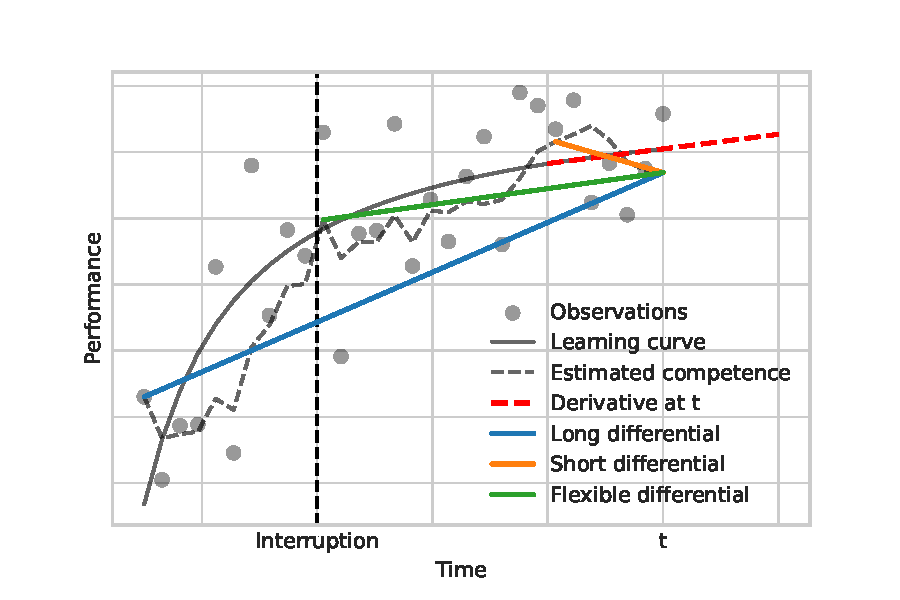
\includegraphics[width=.8\linewidth]{Figures/c5/lptw.pdf}}
    \caption[short figure description]{\textbf{Temporal extent of \ac{LP} estimation}. The plot depicts a hypothetical learning curve on which performance increases with diminishing returns over time. The derivative of this curve represents the true rate of improvement. The learner does not know neither the true learning curve nor its derivative. However, learners compare the estimated performance values at different points in time. Here, the dashed curve represents the box-car estimated learning curve derived from noisy observations (black dots). Note that learning is interrupted for an unspecified period of time (dashed vertical line). Comparing current performance with a very distant reference point is likely to overestimate the derivative (blue line). Comparing it to reference points that are too close in time is unreliable, given the noise in observations (orange line). Resetting the reference point to the beginning of the current episode is more likely to be accurate, if enough attempts are made during the episode (green line).}\label{fig:5-lptw}
\end{figure}

%This situation is similar to the bias-variance tradeoff in statistics and \ac{ML}. While humans might prefer high-bias and low-variance estimates when it come to predicting uncertain quantities \cite{gigerenzer_heuristics_2011}, a more precise specification would be useful.

% Flexible referencing
Fixed time-window computation might be too restrictive to account for the diversity of learning trajectories across different tasks. Shorter time windows are more useful for easier tasks where learning progresses rapidly, while longer time windows are more appropriate for more slowly developing skills. Fixed time-window computation also requires ad hoc assumptions to handle situations in which the reference point extends beyond what is available. For example, given a time window of size $\tau$, the learner would require at least $\tau$ performance evaluations to compute \ac{LP}, unless the parameter is allowed to vary in the beginning. A more flexible approach would be to reset the reference point to when the task is switched to. Such an approach raises the question of how task-disengagement is decided. It turns the relationship between \ac{LP} and its temporal extent upside down: instead of \ac{LP} depending on the fixed time window, the temporal extent of \ac{LP} judgments would depend on the rate of learning (assuming that low \ac{LP} signals the need to disengage from the current task). This temporally flexible \ac{LP} estimation approach is assumed by the psychological \emph{Region of Proximal Learning} theory \parencite{metcalfe_region_2005}, which proposes that once a task is chosen, the amount of time spent on the task will depend on subjective \ac{LP}.

% Summary
In summary, we want to explore the idea that in tasks lacking clear performance feedback (such as precise success rates), \ac{LP} computation is based on performance data that learners decide to monitor. Such data may not correspond to our preconceived objective criteria, so it needs to be validated empirically. What measures learners consider is only one piece of a puzzle. To understand \ac{LP} computation more fully, we also need to understand what they compare the monitored measures to (the question of temporal extent of \ac{LP} estimation). The next section describes an ongoing scientific project aiming to address these questions.

\section{Empirical Study of Improvement Judgments}
One approach to study the computational tenets of metacognitive judgments of improvement is by observing how subjective self-evaluations change over the course of practicing a skill. To increase the ecological validity of the results, we want to emulate a naturalistic learning process which is extended in time, interrupted by other daily activities, and does not feature advanced external performance information. To meet these demands, we have designed a sensorimotor learning activity presented to participants as a video game, called \emph{Lunar Lander}. The goal of the game is to guide a spacecraft (the "lander") onto a landing platform in a controlled manner, so that it does not crash on impact with the ground or go off-screen. To probe participants' subjective judgments about their performance, we solicit the corresponding verbal reports. The secondary objective of the study is to evaluate the impact of subjective judgments of performance dynamics on the motivation to engage in the task. For this, we employ existing verbal psychometric instruments and behavioral techniques for measuring intrinsic motivation.

\subsection{The Lunar Lander Game Task}

% Background
The task is based on a famous arcade video game \parencite{LunarLander19792021}. Using the Box2D physics engine in JavaScript, we implemented a custom version of the game (see Fig. \ref{fig:5-ll_ss}) in order to control the game difficulty and to be able to record the game play. Like the original, our version features a controllable spacecraft and a randomly generated uneven terrain (see Figure). The game is played across multiple trials. Within a single trial, there is a constant gravity vector that can point directly downward or be slanted in order to create an impression of constant wind. We used a variable time differential to simulate the game physics. This ensured that the animation adapts to the user display's frame rate in order to keep the gameplay consistent across users \parencite{fiedler_fix_2004}. Thus, game states were sampled at a constant rate of 80 Hertz.

\begin{figure}[bth]
    \centering
    {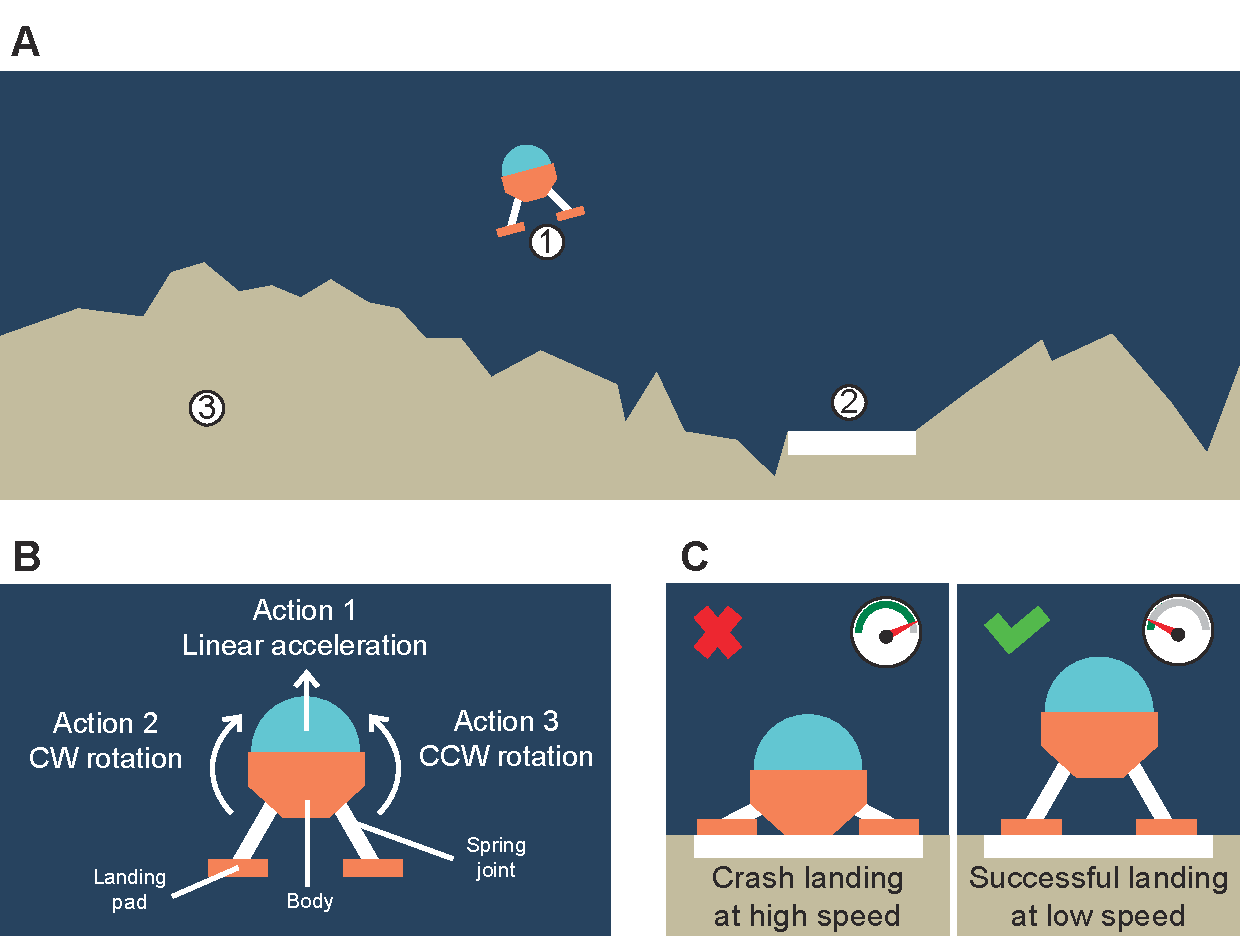
\includegraphics[width=\linewidth]{Figures/c5/ll_ss.pdf}}
    \caption[short figure description]{\textbf{The Lunar Lander game}. \textbf{A}, A single frame from a game trial. The spacecraft \circled{1} is controlled by the player to land it onto the platform \circled{2} and avoid crashing into the terrain \circled{3}. The crashing event is triggered whenever the body of the lander (see \textbf{B}) collides with any other object in the environment, including the spacecraft's own landing pads. \textbf{B}, The spacecraft (consisting of the body, two spring joints, and two landing pads) can be controlled by 3 actions: linear acceleration, and clockwise/counterclockwise rotation. \textbf{C}, Successful landing requires placing the spacecraft (landing pads down) at a sufficiently low speed. Even if a player successfully drives the spacecraft to the landing platform, exceedingly high speed causes the spring joints to compress, resulting in a crash.}\label{fig:5-ll_ss}
\end{figure}

% Gameplay
Each trial of the game ends in one of three outcomes. The spacecraft can go off-screen, in which case, the player is informed that the lander has been lost. The body of the spacecraft can make contact with the ground, in which case is informed that the lander has been crashed. Finally, if the spacecraft can be landed by being carefully placed onto the landing platform (landing pods down) and being kept there for 3 seconds, in which case the player is informed that the lander has successfully landed. The legs of the lander to which the landing pods attach are implemented as spring joints that can be compressed under a force. Thus, the momentum of the spacecraft must be controlled upon landing, even if the spacecraft descends in an upright angle; otherwise the legs will over-compress and the lander will crash.

% Controls
The spacecraft can be controlled by 3 actions (4, if we count doing nothing as an action). Players can rotate the lander clockwise or counter-clockwise and propel it linearly in the direction of the longitudinal axis. Under the hood, actions apply impulse to different points on the spacecraft body. Since there is no friction, stopping or slowing down the angular motion of the body in one direction requires applying an impulse in the opposite direction. Pressing and holding an action key amounts to applying the corresponding impulse on each cycle of the physics simulation, making the spacecraft gain momentum very quickly. Mastering the game requires learning to control the spacecraft, which entails understanding the effects of actions in various contexts. Specifically, learning the game physics requires improving predictions about the velocity of the spacecraft, given the applied actions and the existing momentum.

% Difficulty control: Lander
There are several parameters that determine the difficulty of the game. We can manipulate the rigidity of the leg joints, which determines the speed with which the spacecraft can be landed safely. We can also manipulate the amount of force exerted on the spacecraft by actions. Increasing these forces makes it easy to lose control over the spacecraft, and decreasing them makes the spacecraft very inert and unresponsive. It is also possible to apply noise to actions to simulate control stochasticity.

% Difficulty control: Initialization
In addition to manipulating the lander parameters, we can also control the environment initialization. For example, we can control the initialization distance between the lander and the platform. Traversing more space might be more challenging. We can also change the width of the landing platform, as well as its height relative to surrounding terrain. Finally, we can control the gravity of the environment, parameterized by vertical and horizontal forces on movable objects. By manipulating the horizontal force, we can create a wind effect that drags the lander to one side of the screen and not just downwards. In the pilot study reported below, we experimented with some of these initialization parameters in order to see their effect on average rates of different outcomes.

\subsection{Performance and Improvement Measures}

% A need for scale validation
To measure people's subjective judgments of improvement, we will ask participants to verbally report their feelings on a numerical scale. To the best of our knowledge, no empirically validated psychometric scale for measuring progress judgments exists. Therefore, there is a need for designing an original scale, which entails initial experimentation with multiple candidate questions to assess their mutual and internal consistencies \parencite{kline_psychological_2005,mcneish_thanks_2018}. This can be done in a separate study aimed specifically at engineering a psychometric instrument for reliable and valid measurement of \ac{LP}.

% Different kinds of LP
Improvement judgments can be instantaneous and prospective. Instantaneous judgments report how much improvement is experienced by the learner at the time when the judgment is made (e.g., "I am making progress"). In contrast, prospective judgments correspond to feelings of expected improvement, if the task was practiced for some additional period of time (e.g., "I can improve if I practice more"). How these kinds of judgments relate to each other and what effect they have on motivation has not been extensively studied before. Therefore, we want to design an instrument capable of measuring each kind of judgment.

% Subjective and objective measures
Although the primary goal is to model improvement judgments using objectively observed measures of performance, it would be useful to periodically collect people's subjective judgments of competence, effort, and difficulty. This can be accomplished efficiently by administering (a part of) the NASA-TLX questionnaire \cite{hart_development_1988} several times during practice. NASA-TLX measures 7 components of the task load, including: 
\begin{enumerate}
  \item Mental demand
  \item Physical demand
  \item Temporal demand
  \item Performance
  \item Effort
\end{enumerate}
We will statistically model performance scores using the hypothesized subjective components of competence (see \autoref{subsec:pilot}). Additionally, to get a better idea of what determines instantaneous and prospective judgments of improvement, we will fit regression models of these judgments as a function of combined measures of performance and task load, followed by model comparisons. 

\paragraph{Intrinsic Motivation Measures}

% SIMS
In order to assess the potential effects of \ac{LP} judgments and other subjective/objective measures of performance on motivation, we need a good tool for measuring it. Luckily, several established approaches exist. For example, the \acf{SIMS} scale \parencite{guay_assessment_2000} measures 4 distinct components of motivation:
\begin{enumerate}
  \item Intrinsic Motivation (IM)
  \item Identified Regulation (IR)
  \item External Regulation (ER)
  \item Amotivation (Am)
\end{enumerate}
The \ac{SIMS}-IM component assesses the extent to which an activity is evaluated as interesting, pleasant, and fun. The \ac{SIMS}-IR subscale measures the importance of the activity to the individual. The score on the \ac{SIMS}-ER scale indicates the extent to which the individual feels coerced into doing the activity (by external forces). Finally, \ac{SIMS}-Am measures the individual's unwillingness to participate in an activity. \ac{SIMS} was proposed as an alternative to the \acf{IMI} \parencite{mcauley_psychometric_1989}, criticized for certain conceptual issues \parencite{guay_assessment_2000}. Despite these issues \ac{IMI} components have good psychometric characteristics and can provide useful measurements beyond intrinsic motivation. While the pilot study reported below does not rely on \ac{IMI}, it certainly has utility for future work.

Another option is to use certain components of the \acf{MSLQ} instrument, e.g., \parencite{duncan_motivated_2015}:
\begin{enumerate}
  \item Extrinsic Goal Orientation (EGO)
  \item Task Value (TV)
  \item Control of Learning Beliefs (CLB)
  \item Self-Efficacy for Learning and Performance (SELP)
\end{enumerate}
The \ac{MSLQ}-EGO subscale measures how much learners desire to accomplish goals that are separable from mastering the activity per se (e.g., demonstrating competence to others). \ac{MSLQ}-TV captures the extent to which learners believe the learning or accomplishing task to be somehow beneficial for them. Task value is sometimes considered a component of intrinsic motivation construct \cite{mcauley_psychometric_1989}. By reporting \ac{MSLQ}-CLB, learners indicate how much they believe that their effort in learning the activity can actually make them learn it. Finally, \ac{MSLQ}-SELP reflects the belief that the task can be mastered eventually, time constraints aside. Conceptually, it is similar to the notion of prospective learning judgments introduced above. One challenge of adopting \ac{MSLQ} subscales is that they were originally designed for classroom settings. Many questions ask the respondents about courses/classes, their contents, assignments, teachings etc. 

% Free choice measure
In addition to the self-reported measures of motivation, we will incorporate a behavioral measure of intrinsic motivation using the free-choice technique \parencite{ryan_self-determination_2000}. After finishing game practice and questionnaires, participants will be offered a free choice between finishing the session or engaging in more game practice. We will then assess the relationship between subjective/objective improvement and their motivation (either acceptance rate or time of additional practice) to engage in the task when they do not have to. 

\subsection{Pilot Study}\label{subsec:pilot}

% Goals of the pilot study
The goals of the first pilot run of our study were (1) to assess the effects of game initialization parameters on task achievement, (2) to explore the relationships between several performance measures and improvement judgments, and (3) to explore the relationships between improvement judgments and motivation.

% Experiment procedure
\begin{figure}[bth]
    \centering
    {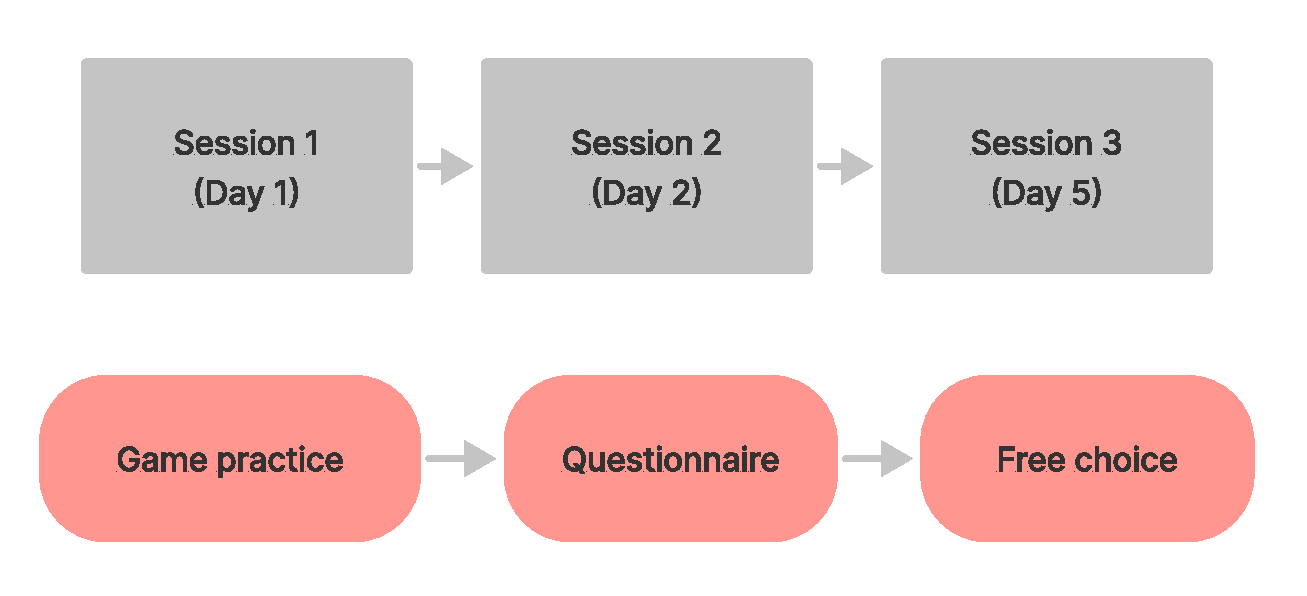
\includegraphics[width=\linewidth]{Figures/c5/procedure.pdf}}
    \caption[short figure description]{\textbf{Pilot experiment procedure}. Participants completed 3 sessions, each on a different day (top row). Each session consisted of game practice, followed by a questionnaire, and a free choice task (bottom row).}\label{fig:5-procedure}
\end{figure}

\subsubsection{Procedure} 
We asked participants ($N=54$) to practice the game over 3 sessions that spanned 5 days. Due to the pandemic caused by COVID-19 outbreak, the pilot experiment was conducted remotely through a custom-designed online platform. We used a fixed schedule for all participants: session 1 was completed on day 1, session 2 on day 2, and session 3 on day 5. Thus, there was 1 day between sessions 1 and 2; and 3 days between sessions 2 and 5. Each session consisted of 3 phases: task practice, questionnaire, and free-choice task (Fig. \ref{fig:5-procedure}). The study was approved by Inria's Operational Committee for the Evaluation of Legal and Ethical Risks (OCELER).

% Two practice durations
Participants played multiple trials of Lunar Lander during the task practice phase. As a precaution from a potential floor/ceiling effect, we asked some participants to practice for 10 minutes, and others for 20 minutes, in each session. In the beginning of each session, participants read through the same instructions about the goal, the rules, and the controls of the game.

% Questionnaire and free choice
After finishing the practice phase, participants were asked to fill in a questionnaire consisting of performance-improvement, NASA-TLX, \ac{SIMS}, and \ac{MSLQ} questions. Full lists of adapted questions can be found in the Appendix (\autoref{ch5-appendix}). After finishing the questionnaire phase, participants were informed that they have finished the session and that they could practice more if they wanted or move on from our task.

\subsubsection{Findings}

\paragraph{Task achievement}

% Success rates across sessions
\begin{figure}[t]
    \centering
    {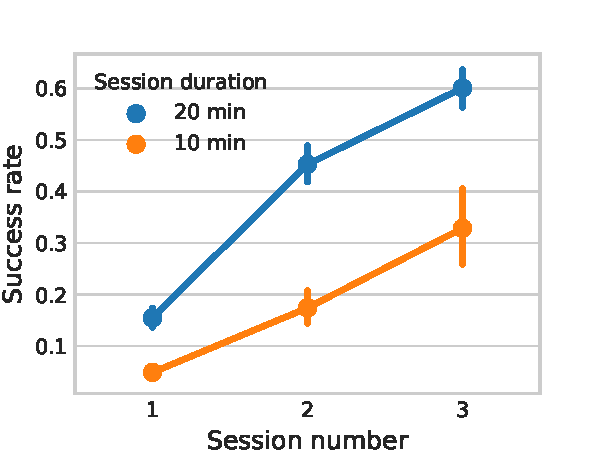
\includegraphics[width=.5\linewidth]{Figures/c5/success_rates.pdf}}
    \caption[short figure description]{\textbf{Success rates across sessions and session durations}. The points represent success rates in the 10-minute (blue) and the 20-minute (orange) condition. Error bars show 95\% CI (the increasing intervals for later sessions are due to participant dropout). Success rates increased steadily in both 10-minute and 20-minute conditions. More time per session allowed participants to perform better, but performance increased almost linearly with each successive practice session, regardless of the duration. Low levels of success in the 10-minute group suggests a floor effect.}\label{fig:5-success_rates}
\end{figure}

% Effects of time on success rate
To get a general sense for the difficulty of the game, we analyzed the success rates across the three practice sessions for the two session-duration conditions (10 minutes and 20 minutes). We fitted a logistic regression of binary trial outcome (success vs. crash/off-screen) as a function of session duration, session number, and their interaction (setting the 10-minute session 2 as the reference group). As shown in Fig. \ref{fig:5-success_rates}, success rates in 20-minute sessions were higher compared to 10-minute sessions. The logistic model predicted the odds of success in a 20-minute (second) session to be 3.924 times higher compared to a 10-minute (second) session (\ac{OR} $=3.924$, 95\% CI $=[3.017, 5.105]$, $z(4654)=10.189$, $p<.001$). Success odds were also significantly different across sessions: compared to the 2nd (10-minute) session, participants were less likely to land during the 1st (10-minute) session (\ac{OR} $=0.244$, 95\% CI $=[0.174, 0.343]$, $z(4654)=-8.137$, $p<.001$) and more likely to land in the 3rd (10-minute) session (\ac{OR} $=2.32$, 95\% CI $=[1.538, 3.505]$, $z(4654)=4.008$, $p<.001$). There was no interaction between session duration and session number, suggesting that participants improved consistently across sessions within each session-duration group. The analysis also advises against restricting the practice to 10 minutes per session, especially for the 1st session. where only about 5\% of all trials were successful. This floor effect might complicate assessing the relationship between performance improvement and subjective judgments of \ac{LP}.  

% Effects of continuous covariates on success rates
\begin{figure}[t]
    \centering
    {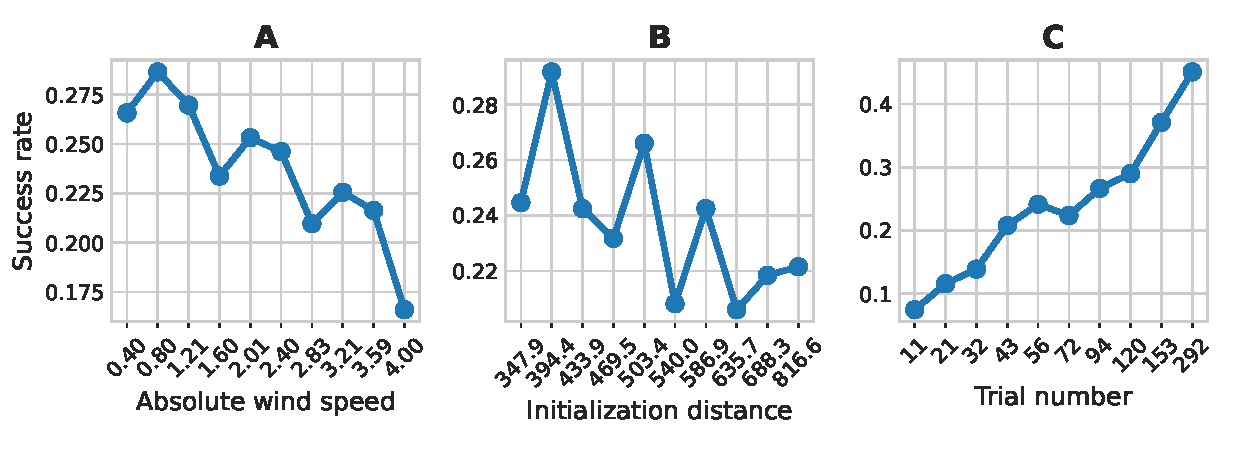
\includegraphics[width=\linewidth]{Figures/c5/init_param_effects.pdf}}
    \caption[short figure description]{\textbf{Success rate covariates}. The three panels show the proportion of successful trials across respective covariates quantized into 10 bins (values on the $x$-axes show quantile upper bounds). \textbf{A} shows the negative correspondence between success rate and the absolute value of the wind parameter. \textbf{B} shows the negative relationship between success rate and initialization distance between the lander and the platform. \textbf{C} shows how average success rates increased over time across sessions. In the range of the first 300 trials, the population-level success rate appears to be increasing linearly with the number of attempts.}\label{fig:5-init_param_effects}
\end{figure}

% Wind and initialization distance
Next, we looked at the effects of game initialization parameters on success (see Fig. \ref{fig:5-init_param_effects}). We fitted a logistic regression of trial outcome as a function of two initialization variables: the absolute wind speed and the initialization distance to the platform; we also included the trial number (cumulative across sessions) as a control variable. To compare the effects, we standardized the regression coefficients by $z$-scoring the covariates. We only included trials from participants who had at least one successful attempt across all sessions played. All three predictors had coefficients significantly different from zero. Thus, accounting for the increasing odds of success over time (\ac{OR} $=1.627$, 95\% CI$=[1.518, 1.743]$, $z(3, 3623) = 13.871$, $p = 001$), participants were less likely to land under a stronger wind (\ac{OR} $=0.821$, 95\% CI$=[0.762, 0.884]$, $z(3623) = -5.249$, $p<.001$) and when initialized farther from the target (\ac{OR} $=0.882$, 95\% CI$=[0.819, 0.949]$, $z(3623) = -3.339$, $p<.001$).

The results reported in this section provide empirical validation for the predicted relationship between the two game-initialization parameters and task difficulty. Thus, it is viable to manipulate these parameters in the future, if we want to control how people learn the task. Figures \ref{fig:5-success_rates} and \ref{fig:5-init_param_effects} (C) also confirm that participants were able to improve over time (at least on a group level), making it viable to study subjective improvement judgments.

\paragraph{Judgments of improvement}

% JOLD questions
At the end of each game-practice session, we asked participants several questions about their subjective improvement. One question probed the retrospective improvement judgment: "Rate how much your current level of performance has changed \textit{compared to the beginning of today's session}". Participants responded by moving an interactive slider along a discrete 11-point semantic differential scale ranging between two polar response categories: "Much worse" (-5) and "Much better" (5); putting the slider at the center of the scale was assumed to indicate the reporting of no perceived change in performance. The same response scale was used to yield a prospective improvement judgment, prompted by "Rate how much you expect to improve over the next session". We explored how self-reported feelings of retrospective and prospective improvement related to different aspects of performance.

% Correlation between prospective and retrospective judgments
\begin{figure}[bth]
    \centering
    {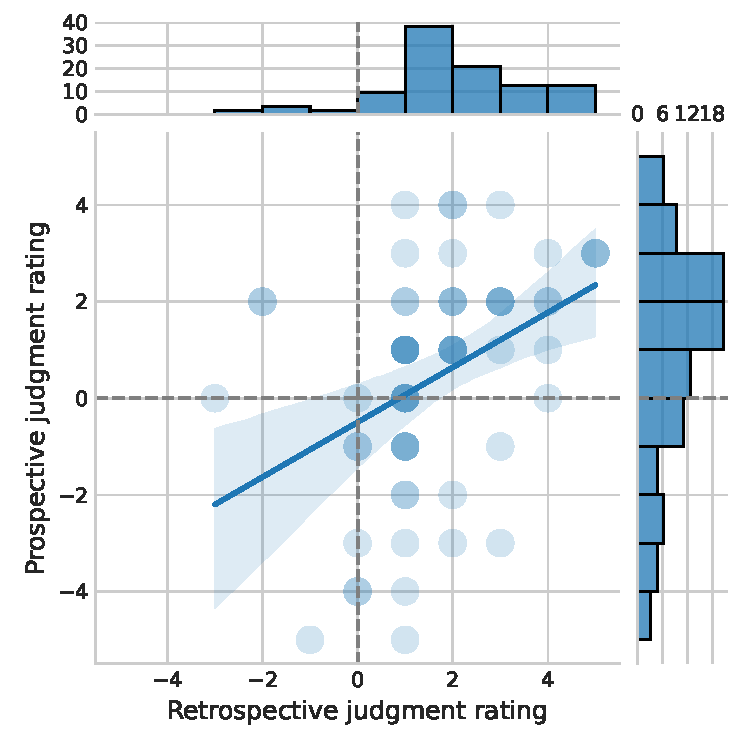
\includegraphics[width=.6\linewidth]{Figures/c5/jolds_corr.pdf}}
    \caption[short figure description]{\textbf{Retrospective and prospective judgments}. The central panel shows the joint distribution of retrospective and prospective improvement judgments. More saturated circles indicate the greater amount of overlapping data points. The line represents a fitted linear regression of prospective judgments on retrospective judgments (the shaded area shows the 95\% CI of the model) The marginal histograms show relative frequencies (\%) of self-reported scores.}\label{fig:5-jolds_corr}
\end{figure}

% Relationship between retrospective and prospective judgments
Fig. \ref{fig:5-jolds_corr} shows the joint sample distribution between retrospective and prospective improvement judgments. There were a total of 63 observations (22 out of 85 prospective-improvement judgments were lost due to data collection error). The marginal histograms show that improvement judgments were mostly positive. However, participants judged their future improvement, compared to how they thought they had previously improved, as indicated by a longer tail into the negative range of the prospective judgment scale. Spearman's correlation coefficient between prospective and retrospective judgments was moderate ($r_{\mathrm{Spearman}}(61) = .491,\ p < .001$). Thus, retrospective feelings of improvement seem to explain some of the variance in prospective progress judgments.

% JOLDs ~ incrase in success rate
Next, we investigated how the dynamics of task-achievement feedback related to the subjective judgments of improvement. For each subject and for each session, we calculated the success rate in the first and the second half of the session and then subtracted the latter from the former (a positive difference indicates improvement). Fig. \ref{fig:5-jolds_1_8_and_srd} depicts relationships between retrospective/prospective improvement judgments and changes in success rates in the corresponding session. Increasing rates of success predicted the retrospective improvement judgments, but not the prospective improvement judgments (see explanation for Fig. \ref{fig:5-jolds_1_8_and_srd}).

% Improvement and success rate difference
\begin{figure}[tbh]
    \centering
    {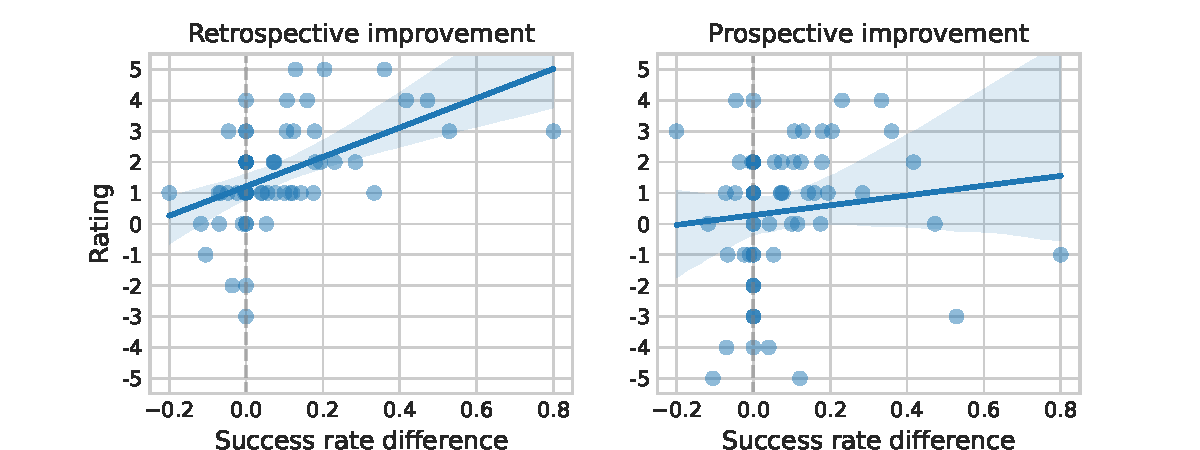
\includegraphics[width=\linewidth]{Figures/c5/jolds_1_8_and_srd.pdf}}
    \caption[short figure description]{\textbf{Increasing success rate predicts self-reported past improvement, but not the expected future improvement}. The circles represent individual data points. The lines represent linear regression models of retrospective and prospective improvement ratings, respectively. The shaded regions represent 95\% CI of the models' predictions. Objective performance improvement, indexed by increasing success rates, reliably predicted the retrospective judgments (slope $=4.728$, 95\% CI $=[2.298, 7.158]$, $t(83) = 3.870$, $p<.001$) but not the prospective judgments (slope $=0.811$, 95\% CI $=[-2.723, 4.345]$, $t(61) = 0.459$, $p=.648$).}\label{fig:5-jolds_1_8_and_srd}
\end{figure}

% Different time scales for LP judgments
In addition to asking participants to rate their improvement within a single session, we asked them to provide more judgments about a more extended period of time. After sessions 2 and 3, we asked participants to compare their performance on the most recent session with their performance on a session just before it (improvement over consecutive sessions). After the 3rd (and last) practice session, we asked participants to also report how their subjective performance improved relative to "the start of the experiment". Due to participant dropout on sessions 2 and 3, we did not collect as much data on these judgments, yet the smaller sample sizes ($N=39$ for session 2, and $N=13$ for session 3) were sufficient to reveal some significant relationships between changes in objective and subjective self-assessments of competence and their corresponding subjective evaluations (Fig. \ref{fig:5-jolds_vs_subjective_objective_competence}, top row). Objective improvement between consecutive session was defined as the difference between success rates in the latest session vs. the session before (positive values indicate improvement). Objective improvement between session 1 and 3 was defined similarly by subtracting the success rate on session 1 from the success rate on session 3. As the top row of Fig. \ref{fig:5-jolds_vs_subjective_objective_competence} illustrates, participant's subjective judgments corresponded relatively well with their objective improvement. We can also see a ceiling effect for the subjective ratings, which could be obscuring the true effect size. At this point, it is difficult to say whether these longer-term judgments are better correlated with objective performance than judgments about within-session learning, but we can say that they are \emph{at least} as well correlated. To determine the time-extent of improvement judgments that are most accurate in relation to success rate, future iterations of the study might benefit from a better-designed instrumentation and a more appropriate scale for measuring subjective improvement.

\begin{table}
    \myfloatalign
    \begin{tabularx}{\textwidth}{XXccccc} \toprule
    Judgment timescale            & Difference in         & \beta  & 95\% CI                 & $t$     & $p$              \\
    \hline
    Consecutive sessions & Success rate          & 1.288  & [0.805, 1.771] & 5.406 & \textless .001 \\
                         & Subjective competence & 1.129  & [0.604, 1.655] & 4.359 & \textless .001 \\
    Sessions 1 and 3     & Success rate          & 0.989  & [0.318, 1.660] & 3.244 & .008           \\
                         & Subjective competence & 0.901  & [0.177, 1.624] & 2.740 & .019           \\ \hline
    \end{tabularx}
    
    \caption[short table description]{Standardized coefficient values from linear regressions predicting subjective improvement judgments  separately for 2 timescales) from differences in success rates or self-reported competence judgments. For the timescale of consecutive sessions (improvement/differences regarding performance on two consecutive sessions), the degrees of freedom for the $t$ test are (1, 37). For the longer timescale (sessions 1 and 3) the degrees of freedom are (1, 11).}  \label{tab:5-jold_2_3_separate_regressions}
\end{table}

% JOLDs and subjective performance measures
Since we did not collect subjective competence ratings \emph{during} the self-paced practice, we could not assess the relationship between the dynamics of subjective competence ratings within sessions and the improvement judgments at the end of each session. However, we did ask people to reflect on their perceived competence once \emph{after} each practice session using an item from the NASA-TLX instrument. Like with success rates, we calculated two kinds of contrasts of self-reported competence scores: one comparing scores from consecutive sessions (Fig. \ref{fig:5-jolds_vs_subjective_objective_competence}, bottom left), and one comparing sessions 1 and 3 (Fig. \ref{fig:5-jolds_vs_subjective_objective_competence}, bottom right). We then explored how improvement judgments related to differences in objective and subjective measures of competence. As shown in Tab. \ref{tab:5-jold_2_3_separate_regressions}, when considered separately, subjective and objective competence differences predicted the corresponding improvement judgments. However, when included in the same model, the results were different for the shorter term improvement judgments (consecutive sessions) compared to the longer-term ones (session 1 vs session 3). Specifically, when modeling self-reported improvement between consecutive sessions, objective difference in success rates appears to be a better predictor ($\beta = 1.003$, 95\% CI = [0.282, 1.724], $t(36) = 2.821$, $p = .008$) than the difference in subjective competence judgments ($\beta = 0.384$, 95\% CI = [-0.337, 1.105], $t(36) = 1.081$, $p = .287$). Neither predictor was significantly different from 0 when regressing the improvement judgments for sessions 1 and 3, but the very limited sample size for this analysis prevents us from drawing any conclusions. These results suggest that people's retrospective judgments of session-to-session improvement are better calibrated to the objective improvement than to the change in subjective competence. Interestingly, self-reported prospective improvement (predicted for the next session) was significantly correlated with the session-to-session change in subjective competence (Spearman's $\rho(23) = .445$, 95\% CI = [.041, .724], $p = .026$), but not with the corresponding change in objective success rates ($p = .155$). It is not obvious why prospective judgments should be better calibrated with the change in subjective competence ratings, while retrospective judgments should be better aligned with objective improvement. This pattern of findings calls for replication and further research, especially considering past research \parencite{townsend_metacognitive_2011} that presents results conflicting with ours.

\begin{figure}[h!]
    \centering
    {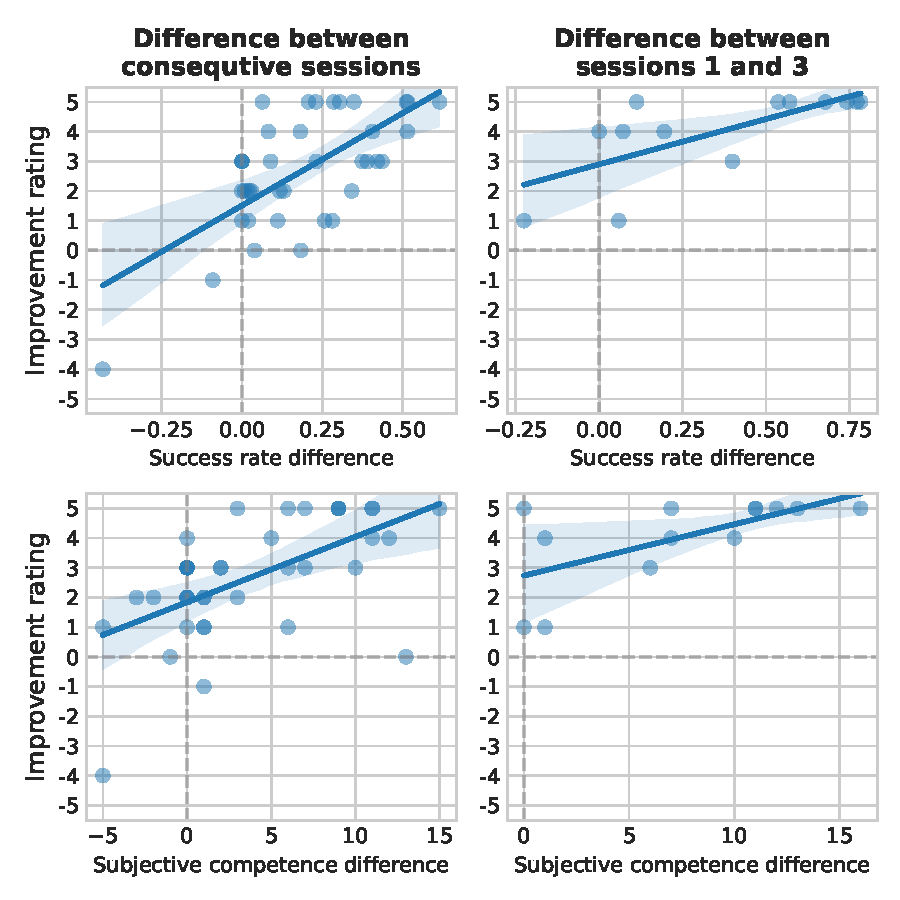
\includegraphics[width=.9\linewidth]{Figures/c5/jolds_vs_subjective_objective_competence.pdf}}
    \caption[short figure description]{\textbf{Subjective and objective changes in competence between sessions predict self-rated improvement}. The circles represent individual data points.The lines represent linear regression models of retrospective shorter-term and longer-term improvement ratings, respectively. The shaded regions represent 95\% CI of the models' predictions. The top row plots differences in success rates against the corresponding improvement ratings. The bottom row shows how difference in subjective competence evaluations relate to judgments of improvement. When considered separately, objective success-rate difference and subjective-competence difference are significantly correlated with improvement judgments, regardless of whether the difference/improvement judgment concerns consecutive sessions or sessions 1 and 3. However, when factored in together, objective success rate appears to be a better predictor for the shorter term judgment.}\label{fig:5-jolds_vs_subjective_objective_competence}
\end{figure}

% The need to look at ohter performance measures
Before proceeding to the next set of results, we would like to note that out of 46 participants, 14 ($30.43\%$) reported positive improvement despite failing to succeed even once\footnote{We report the results from 46 (not 54) participants, because 8 out of 54 participants dropped out immediately after completing the 1st game practice without filling in the questionnaires.}. Some participants reported positive improvement while showing a negative change in their success rate. This could be interpreted in at least two different ways. One possibility is that while people base recent improvement judgments on success-rate dynamics, their self-reported ratings of improvement are unreliable due to metacognitive miscalibration. Another explanation is that improvement self-reports can be accounted for by something other than task-achievement feedback. Either way, there is a need to investigate the residual variation in improvement judgments that is beyond what can be explained by changing success rates or subjective performance evaluations. For if we want to assess metacognitive accuracy -- we need to identify the set of valid objective measures that subjective improvement is based on, and there are no a priori reasons to assume that this set includes only the task-achievement feedback. Investigating how \ac{LP} judgments arise, especially prior to witnessing task achievement, is an important direction for future research.

% Attempts to find non-binary performance indicators
Here, we experimented with several performance-relevant variables. For each trial, we computed the weighted-average\footnote{More weight was assigned to values closer to the end of a trial} distance, vertical speed, and horizontal speed, and then regressed these variables on the trial number in order to obtain slope coefficients describing how each variable changed throughout sessions. For instance, a negative slope for the weighted-average distance variable would indicate that the average-distance to the platform decreased over the course of the session, potentially signaling gradual improvement in performance. When considered together with success-rate difference scores, weighted-average distance and speeds were not reliably associated with judgments of improvement. This negative result motivates a search for performance indicators that learners might use in order to self-assess beyond success rates. An intriguing lead to pursue in the future is the subjective evaluation of sensorimotor control -- people might report improvement when they feel more control. 

\paragraph{Motivation and learning beliefs}
Next, we explored how different operationalizations of \ac{LP}, such as changes in objective/subjective competence and subjective improvement judgments, related to various attitudes regarding our sensorimotor game-task. Specifically, we computed Spearman's correlation coefficients between each measure of \ac{LP} and different motivational and attitudinal variables measured by \ac{SIMS} and \ac{MSLQ} (see Fig. \ref{fig:5-motivation_corrs_tight}). As it is impossible to infer causality from these correlations, future iterations of the study will benefit from measuring motivation and learning beliefs before and after task practice. Below, we provide only speculative interpretations of the results in the figure.

\begin{figure}[tbh]
    \centering
    {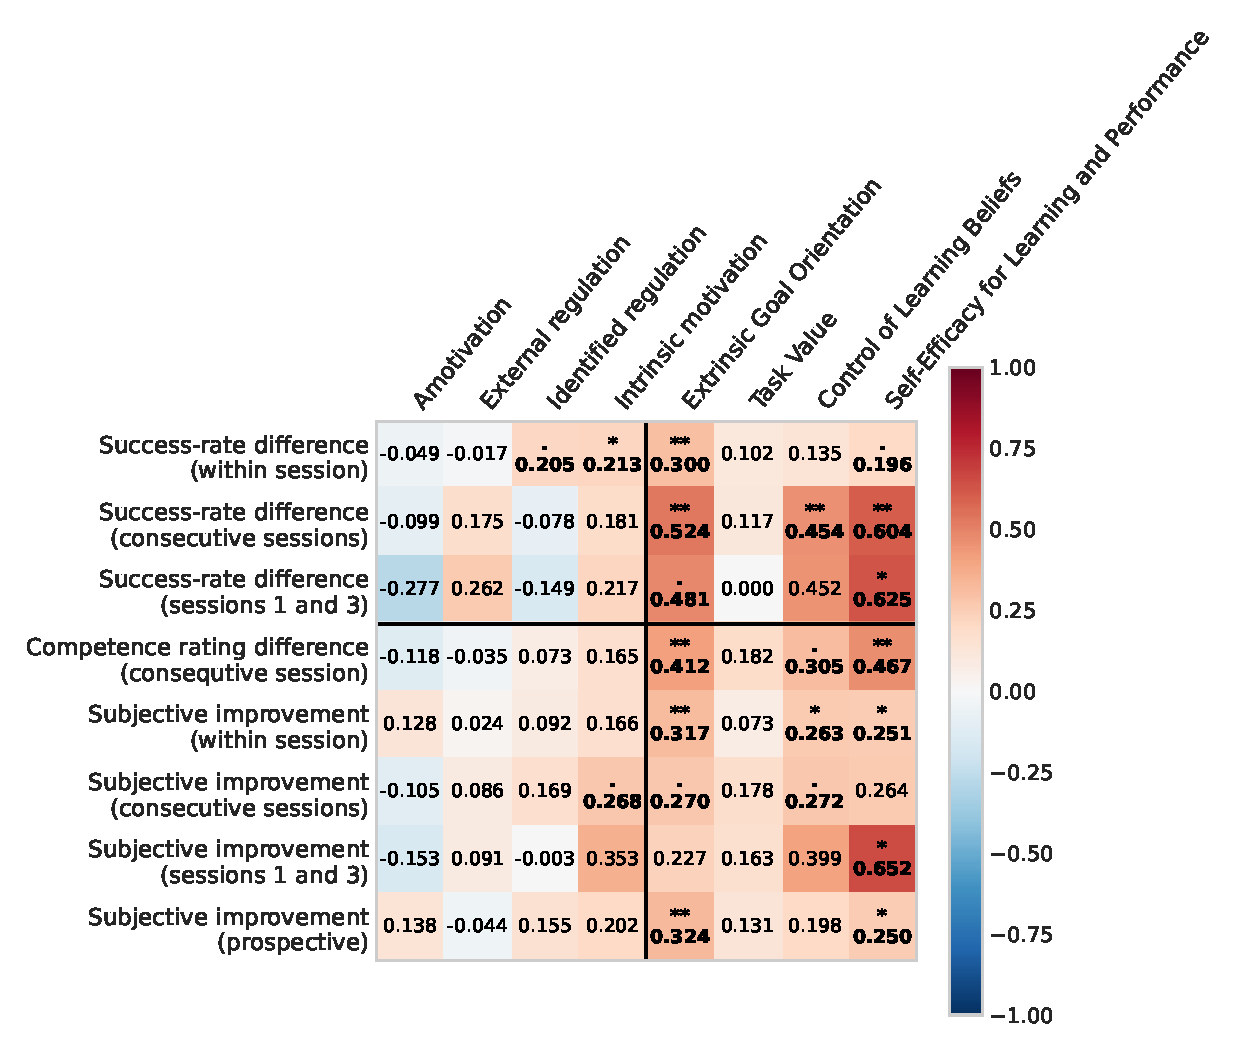
\includegraphics[width=.9\linewidth]{Figures/c5/motivation_corrs_tight.pdf}}
    \caption[short figure description]{\textbf{Correlations between different operationalizations of
    \ac{LP} and motivation}. Each cell shows the value of a Spearman's correlation coefficient. '.' indicates that the $p$-value for the coefficient is between $.05$ and $.10$; '*' indicates a $p$-value of less than $.05$; '**' indicates a $p$-value of less than $.01$. The black vertical line separates \ac{SIMS} items (1st 4 columns) from \ac{MSLQ} items (last 4 columns). The black horizontal line separates objective behavioral measures of \ac{LP} from measures based on subjective ratings.}\label{fig:5-motivation_corrs_tight}
\end{figure}

% LP and IM
We were mainly interested in the relationship between \ac{LP} and intrinsic motivation. Our data did not show many significant correlations between the \ac{SIMS}'s Intrinsic Motivation (\ac{SIMS}-IM) measure and any of our measures of \ac{LP}. Despite the lack if statistical significance, \ac{SIMS}-IM scores yielded consistently positive correlation coefficients across different measures of improvement. However, even if the lack of statistical significance is due to the limited sample size, the correspondence between intrinsic motivation and subjective/objective improvement appears to be moderate at best. This result suggests that the relationship between \ac{LP} and (intrinsic) motivation -- if anything -- is not straightforward as sometimes conceived.

% JOLDs and Extrinsic Goal Orientation
Our measures of \ac{LP} correlated more strongly and consistently with 3 out of 4 subscales (that we used) from the \ac{MSLQ} instrument. There were several positive correlations with the Extrinsic Goal Orientation subscale, which measures the extent to which task performance is motivated by extrinsic ends (e.g. impressing or surpassing others). Participants who wanted to do well in the game showed greater objective improvement and were largely aware of it.

% JOLD and Control of Learning Beliefs
Several measures of \ac{LP} also predicted two distinct kinds of beliefs about learning: Control of Learning Beliefs (\ac{MSLQ}-CLB) and Self-Efficacy for Learning and Performance (\ac{MSLQ}-SELP). The first measure reflects a learner's beliefs that being successful in the task depends on his or her efforts. It could be that objective/subjective \ac{LP} fuels such beliefs, but the reverse causality is also possible: believing that one is in control of one's learning could enhance learning. The same is true for the relationship between the self-efficacy measure and \ac{LP}: improving on a task might reinforce the belief that one can eventually perform the task well, but such a belief can also invigorate the learning process. Of course, it is also possible that beliefs about the control of learning and self-efficacy have reciprocal relationships with \ac{LP} whereby \ac{LP} strengthens learning beliefs, which boost motivation, which contributes to \ac{LP}.

% Possible causal relationship between LP and MSLQ-SELP
Additional analyses lend some support to the reciprocity between \ac{LP} on self-efficacy. First, the \ac{MSLQ}-SELP rating given at the end of session 1 was a reliable predictor of the objective improvement from session 1 to session 2 (slope $= 0.070$, 95\% CI $=[0.032, 0.108]$, $t(2, 23) = 3.827$, $p = .001$). Second, the objective improvement from session 1 to session 2 was a reliable predictor of the \ac{MSLQ}-SELP rating given after the 2nd practice session (slope $= 0.907$, 95\% CI $=[0.981, 4.049]$, $t(23) = 3.391$, $p = .003$), while controlling for the same rating from the previous session. Thus, while self-efficacy for learning beliefs predicted objective improvement over consecutive sessions, objective improvement predicted the updated self-efficacy beliefs above and beyond the previous values. Similar analyses did not provide the same support for the reciprocity between \ac{LP} and beliefs about learning control. While the \ac{MSLQ}-CLB ratings from session 1 predicted improvement from session 2 to session 1, this improvement measure failed to predict the 2nd session's ratings beyond what the 1st session's ratings predicted.

% Learning beliefs predict IM
Interestingly, each of the learning-belief measures correlated strongly with the \ac{SIMS}-IM scores (Control of Learning Beliefs: Spearman's $\rho(83) = 0.401$, 95\% CI = $[0.197, 0.571]$, $p < .001$; Self-Efficacy: Spearman's $\rho(83) = 0.552$, 95\% CI $= [0.370, 0.693]$, $p < .001$), suggesting that learning beliefs might mediate the effect of \ac{LP} on intrinsic motivation. Specifically, \ac{LP} might only increase the intrinsic motivation for performing/learning a task if it feeds the belief that the task can and eventually will be learned.

% Success rate
The last set of results concerns a strong predictor of motivation and learning beliefs that is not a measure of \ac{LP}. Our data showed that plain success rates, measured as the proportion of successful trials in a session, predicted most of \ac{SIMS} and \ac{MSLQ} components. Specifically, success rates were negatively correlated with amotivation (\ac{SIMS}-Am; Spearman's $\rho(83) = -0.233$, 95\% CI = $[-0.428, -0.018]$, $p = .031$), and positively correlated with \ac{SIMS}-IM (Spearman's $\rho(83) = 0.374$, 95\% CI = $[0.168, 0.550]$, $p < .001$), extrinsic goal orientation (\ac{MSLQ}-EGO; Spearman's $\rho(83) = 0.513$, 95\% CI = $[0.324, 0.662]$, $p < .001$), task value (\ac{MSLQ}-TV; Spearman's $\rho(83) = 0.256$, 95\% CI = $[0.052, 0.456]$, $p = .014$), \ac{MSLQ}-CLB (Spearman's $\rho(83) = 0.480$, 95\% CI = $[0.286, 0.636]$, $p < .001$), and \ac{MSLQ}-SELP (Spearman's $\rho(83) = 0.693$, 95\% CI = $[0.547, 0.799]$, $p < .001$).

% Success rate predicts behavioral IM
Remarkably, session-wise success rates also predicted whether a participant would accept the free choice of additional practice after finishing the main practice and the questionnaire. This was shown by a logistic regression of the event of accepting optional practice as a function of success rate. Notably, none of the \ac{SIMS}, \ac{MSLQ}, or our \ac{LP} measures reliably predicted the acceptance of optional practice. However, when considered in a multiple logistic regression together with success rate, several measures obtain significant coefficients, including \ac{SIMS}-Am, \ac{SIMS}-IR, \ac{SIMS}-IM, \ac{MSLQ}-TV, and \ac{MSLQ}-SELP (summarized in Tab. \ref{tab:5-multiple_regs}). This suggests that while success rate accounts for much of the variance in the probability of choosing optional practice, the residual variation can be explained by motivational/attitudinal variables.

\begin{table}
    \myfloatalign
    \begin{tabularx}{\textwidth}{Xcccc}
        \toprule
        Measure &   coef & 95\% CI &   $t(82)$  &    $p$ \\
        \hline
        \ac{SIMS}-Am & -0.480 &  [-0.906, -0.055] & -2.213 &  .027 \\
        \ac{SIMS}-IR &  0.562 &    [0.122, 1.002] &  2.505 &  .012 \\
        \ac{SIMS}-IM &  0.486 &    [0.092, 0.879] &  2.419 &  .016 \\
        \ac{MSLQ}-TV &  0.549 &    [0.104, 0.994] &  2.418 &  .016 \\
        \ac{MSLQ}-SELP &  0.631 &     [0.21, 1.053] &  2.935 &  .003 \\
        \hline
    \end{tabularx}
    \caption[short table description]{Significant bivariate logistic regression coefficients. Each row presents the coefficient estimate, the $t$-statistic, and  the $p$-value of a motivational/belief measure that was significant in a multiple logistic regression model of accepting optional practice.}  \label{tab:5-multiple_regs}
\end{table}

% Behavioral IM, success rate and motivaiton
One interpretation is that motivational/attitudinal factors determine decision-making at specific levels of success rate. This possibility was supported by three multiple logistic regression models (of accepting optional practice) that included the success rate, a motivational/attitudinal score, and their interaction. In these models, involving \ac{SIMS}-IR, \ac{SIMS}-IM, and \ac{MSLQ}-SELP, respectively, the coefficients representing the main effects of motivational/attitudinal variables were significant, while the effect of success rate or interaction were not. This means at the success rate of 0, identified regulation, intrinsic motivation, and self-efficacy for learning and performance, predict whether the learner takes on the optional practice. The effects of \ac{SIMS}-IR and \ac{SIMS}-IM are intuitive: personally identifying with an activity and finding it inherently interesting or fun makes one more likely to engage in this activity. The effect of \ac{MSLQ}-SELP is less obvious, but intriguing. It suggests, that when performance is at a low level, one is more likely to engage in practice if one believes that he or she will eventually succeed.

\subsubsection{Pilot Study Discussion}
With this pilot study we wanted to (1) assess the effects of game initialization parameters on task achievement, (2) explore the relationships between several performance measures and improvement judgments, and (3) to explore the relationships between improvement judgments and motivation. The results provide important lessons and pose intriguing questions for future work.

% Summary of results section 1: task difficulty manipulation
First, we have obtained some understanding of how several game parameters affect task-achievement rates. Manipulating objective difficulty is important to test causal relationships between learning and motivation/attitudes. Our results provide useful approximations of the effect sizes of game-difficulty parameters on task achievement. We also gained a sense of the learning dynamics and individual variability for the task. This knowledge can be used for manipulating group-level learning profiles in independent-group designs. Given adequate tools for measuring the relevant data, we should be able to examine how self-evaluated performance dynamics relate to motivation and learning beliefs.

% Summary of results section 2: success rates predict improvement judgments
Our pilot study also showed that people might rely on the objective success-rate and/or subjective-competence dynamics in verbally reporting their improvement. Moreover, competence changes, measured over different temporal intervals, correlated with the corresponding self-reported judgments of improvement. The original intention behind soliciting judgments of improvement about different time intervals was to evaluate whether judgments of some duration(s) would be better calibrated with reality than others, but our analyses failed to reveal such differences. The reported improvement judgments of different temporal sizes were similarly correlated with the corresponding objective improvement measures. It remains to be shown if there is a "basic" temporal interval which people tend to use naturally to gauge improvement for self-regulated learning, or if \ac{LP} is temporally flexible. 

% Townsend and Heit, 2011
Our results suggest that changes in (objective) success rates explain variation in improvement judgments better, compared to changes in subjective evaluations of self-competence. This is not consistent with the results presented by Townsend and Heit \parencite{townsend_judgments_2011,townsend_metacognitive_2011} who found no correlation between changes in objective performance scores and subjective improvement judgments. There are, of course, many potentially important differences between our study and Townsend and Heit's work that might explain the divergence. Most pertinently, Townsend and Heit measured objective performance (or competence) as the percentage of items recalled in the learning set, which might be far from how learners subjectively represent competence in a list-memorization task. In our study, on the other hand, success rate might be a very natural indicator of competence. This points to the importance of understanding how learners evaluate their performance subjectively.
% Moreover, Townsend and Heit measured people's subjective competence as \acp{JOL} common to metamemory research. \acp{JOL} ratings reflect people's subjective estimation of performing the task (recall) in the future. On the other hand, we relied on the task-performance scale from NASA-TLX which is more about one's subjective evaluation of past performance.

% Summary of results section 3: Motivation might depend on leanring beliefs
Finally, we explored how different operationalizations of \ac{LP}, including objective and subjective variables, relate to motivational and attitudinal measures from \ac{SIMS} and \ac{MSLQ}. While \ac{LP} seems to correlate rather weakly with intrinsic motivation, we found it to be a good predictor of beliefs about learning control and self-efficacy. Research in motor-learning regulation \parencite{wulf_optimizing_2016,lewthwaite_optimizing_2017} convincingly shows that increasing self-efficacy and intrinsic motivation has positive effects not only on sensorimotor performance, but also on sensorimotor learning and retention. For example, selectively providing feedback information about the best versus the worst practice attempts enhances self-efficacy and intrinsic motivation during skill acquisition and results in better learning and retention of the skill \parencite{abbas_good-vs_2018}. Our findings are complementary to this literature. First, they show that better learning might be associated with strengthening beliefs that the task can and will be learned, both of which correlate with intrinsic motivation. Second, while the cited literature studies the effects of motivation/attitudes on sensorimotor learning itself, we demonstrate how motivation/attitudes contribute to skill acquisition by guiding decision-making for task engagement.

\section{Concluding remarks}

Although direct and unequivocal demonstration of \ac{LP} computation in humans is still missing, there are compelling theoretical \parencite{son_metacognitive_2006,lopes_strategic_2012,gottlieb_information-seeking_2013} and empirical \parencite{metcalfe_region_2005,poli_infants_2020,ten_humans_2021,leonard_young_2021} reasons to believe that active learning in humans depends on \ac{LP}. On the other hand, metacognition research suggests that human reasoning about their own learning is not always accurate, particularly when it comes to improvement judgments \parencite{townsend_judgments_2011,townsend_metacognitive_2011}. To reconcile the tension between these views, we need not only a good definition (or a comprehensive taxonomy) for the concept of \ac{LP}, but also authentic and reliable measurement tools.

Having reviewed several computational mechanisms of \ac{LP}, this chapter raised two important questions that need to be addressed before we can measure and model subjective \ac{LP}. One question is how do humans subjectively represent tasks and task performance? Measures of \ac{LP} based on the researcher's performance standards may differ from what people consider when judging how well they are doing and if they are improving. Understanding the general principles behind subjective competence representations across different tasks is key to being able to procure valid measurements of subjective performance and performance progress. Another question is, what determines the time extent of progress judgments? Assuming that \ac{LP} computation entails a comparison of one's current state of knowledge to a state in the past, it is not obvious how this comparison is parameterized in humans. Is there a fixed time window that humans compute \ac{LP} over, or do we flexibly allocate our time to practicing particular tasks in order to get reliable \ac{LP} estimates?

We have sketched out some of the main components of a behavioral study that can potentially elucidate the mechanisms of progress metacognition. In it, we emphasize the importance of emulating a naturalistic learning process in which the learner practices an ecologically valid task (a video game) in an ecologically valid way (spaced over several practice sessions spanning multiple days). The pilot study reported above is an important step toward finalizing the exact details of a future study, but other investigations are also due.

As discussed previously, we need a reliable psychometric scale for collecting verbal reports of improvement judgments. Our pilot study explicitly asked people to compare their current level of performance with a reference performance in the past. To solicit a more general sense of improvement, we might benefit from measuring several related indicator variables \parencite{fullmer_psychometrics_2020}, rather than probing specific comparisons. Additionally, future research will benefit from measuring participants' prior beliefs about their performance on the task. This will be useful for evaluating performance-based models of competence belief updating discussed in the beginning of this chapter. 

Most certainly, the investigation of competence and competence progress metacognition will present novel challenges that we have not accounted for so far, but it appears that we possess the right tools for taking the first steps towards understanding this aspect of human cognition.